\documentclass{article}
\title{Informe}
\usepackage[utf8]{inputenc}
\usepackage{algorithm}
\usepackage{algorithmic}
\usepackage{graphicx}
\usepackage{}
\author{David Díaz Jiménez, Andrés Rojas Ortega}

\begin{document}
	
	\begin{figure}[t]
		\centering
		
\includegraphics[scale=0.2]{img/np_UJA_generica_6.png}
		
\includegraphics[scale=0.35]{img/Logo_EPS.png}
		
	\end{figure}
	
	\begin{center}
		
		\begin{large}
			
			Metaheurísticas
			
		\end{large}
		
		\vspace*{0.2in}
		\textbf{\large Informe de prácticas}
		
		\vspace*{.2in}
		
		David Díaz Jiménez, Andrés Rojas Ortega
		
		\vspace*{2.5cm}
		
	\end{center}

	\tableofcontents
	
	\newpage
	
	\section{Definición y análisis del problema}
	
	\paragraph{}Dado un conjunto \emph{N} de tamaño \emph{n}, se pide encontrar un subconjunto \emph{M} de tamaño \emph{m}, que maximice
	la función: 
	
	\[ d(s_i,M)=\sum_{s_j \in M} d(s_i,s_j)\]
	donde  $d(s_i,s_j)$ es la diversidad del elemento $s_i$ respecto al elemento $s_j$
	
	\subsection{Representación de la solución}
	
	\paragraph{} Para representar la solución se ha optado por el uso de un vector de enteros, en el que él elemento contenido en cada posición se corresponde con un integrante de la solución. La solución vendrá dada por las siguientes restricciones:
		\begin{itemize}
			
			\item La solución no puede contener elementos repetidos.
			
			\item Debe tener exactamente \emph{m} elementos.
			
			\item El orden de los elementos es irrelevante.
			
		\end{itemize}
	
	
	\subsection{Función objetivo}
	
	\[ d(s_i,M)=\sum_{s_j \in M} d(s_i,s_j)\]
	
	\subsection{Operadores comunes}
	
	\paragraph{}El operador de intercambio es el 1-opt, se seleccionara un elemento de la solución actual en base a un criterio y se sustituirá por un elemento que no pertenece a la solución. 
	
	\section{Clases auxiliares}
	
	\paragraph{} A continuación se enumeran las diferentes clases auxiliares utilizadas en el programa y una breve descripción de los atributos y funciones que las componen.
	
	\paragraph{nota:}Los constructores, getters y setters se han omitido.
	
	\subsection{Archivo}
	
	\paragraph{}Clase que almacena toda la información que se encuentra dentro de un archivo.
	
	\subsubsection{Atributos}
	
	\paragraph{nombre String:}Nombre del objeto.
	
	\paragraph{ruta String:}Ruta completa del archivo de datos.
	
	\paragraph{tamaMatriz Integer:}Tamaño de la matriz de datos.
	
	\paragraph{tamaSolucion Integer:}Tamaño de la solución.
	
	\paragraph{matriz float[ ][ ]:}Matriz que almacena todos los datos del archivo.
	
	\subsubsection{Funciones}
	
	\paragraph{presentarDatos()}Muestra por pantalla los datos del Archivo y el contenido de matriz.
	
	\subsection{Configurador}
	
	\paragraph{}Clase que almacena todos los parámetros principales del programa.
	
	\subsubsection{Atributos}
	
	\paragraph{directoriosDatos ArrayList$<$String$>$} Almacena los directorios donde se encuentran los archivos con la información del problema.
	
	\paragraph{semilla Long}Semilla utilizada para generar números aleatorios.
	
	\paragraph{iteraciones Integer} Número de iteraciones.
	
	\paragraph{intentosTabu Integer} Número de intentos en la búsqueda tabú para mejorar la solución élite.
	
	\paragraph{iteracionesTabu Integer}Número de iteraciones en la búsqueda tabú.
	
	\paragraph{recuperarSemilla Long} Almacena el valor inicial de la semilla.
	
	\paragraph{tenenciaTabu Integer} Número de ciclos que un elemento se almacena en la lista tabú.
	
	\subsubsection{Funciones}
	
	\paragraph{rotarSemilla()} Rota las posiciones de la semilla una posición a la derecha.
	
	\paragraph{RecuperarSemilla()}Restaura la semilla a su estado original.
	
	\subsection{ElementoSolucion}
	
	\paragraph{}Clase que almacena la información de cada elemento que forma parte de la solución.
	
	\subsubsection{Atributos}
	
	\paragraph{id int}Indica el elemento de la solución que representa.
	
	\paragraph{contribucion float}Coste que aporta el elemento a la solución.
	
	\paragraph{vecesSolucion}Veces que el elemento ha formado parte de la solución.
	
	\subsubsection{Funciones}
	
	\paragraph{compareTo(ElementoSolucion vecino)}Compara dos ElementoSolucion.
	
	\paragraph{toString()}Método toString de la clase.
	
	\subsection{GestorLog}
	
	\paragraph{}Clase encargada de crear y escribir los archivos Log del programa.
	
	\subsubsection{Atributos}
	
	\paragraph{archiveName String} Nombre del archivo en el que escribir
	
	\paragraph{fichero FileWriter} Fichero a escribir.
	
	\paragraph{pw PrintWriter} Encargado de escribir en fichero.
	
	\subsubsection{Funciones}
	
	\paragraph{abrirArchivo()}Abre el archivo archiveName.
	
	\paragraph{escribirArchivo(String linea)}Escribe la información guardada en linea en el archivo.
	
	\paragraph{cerrarArchivo()}Cierra el fichero.
	
	\subsection{Metaheuristicas}
	
	\paragraph{}Clase que calcula todos los resultados con los algoritmos solicitados sobre todos los datos facilitados.
	
	\subsubsection{Atributos}
	
	\paragraph{config Configurador}Contiene los parámetros principales del programa.
	
	\paragraph{nombre String}Nombre del objeto Metaheurísticas.
	
	\paragraph{archivos ArrayList$<$Archivo$>$}Contiene el nombre de los archivos que contienen los datos sobre los que hacer los cálculos.
	
	\paragraph{rutaCarpetaArchivos String}Directorio que contiene los archivos.
	
	\subsubsection{Funciones}
	
	\paragraph{lectorArchivos()}Realiza la lectura de todos los datos de todos los archivos.
	
	\paragraph{mostrarDatos()}Muestra por pantalla los datos de todos los archivos leídos.
	
	\paragraph{greedy()}Calcula la solución para todos los archivos utilizando el algoritmo Greedy y muestra el resultado por pantalla.
	
	\paragraph{busquedaLocal()}Calcula la solución para todos los archivos utilizando el algoritmo de búsqueda local y muestra el resultado por pantalla.
	
	\paragraph{busquedaTabu()}Calcula la solución para todos los archivos utilizando el algoritmo de búsqueda tabú y muestra el resultado por pantalla.
	
	\subsection{Pair}
	
	\paragraph{}Representa un par formado por un candidato y un coste asociado a este.
	
	\subsubsection{Atributos}
	
	\paragraph{candidato Integer} id del candidato almacenado.
	
	\paragraph{coste float} Coste asociado al candidato.
	
	\subsection{RandomP}
	
	\paragraph{}Clase para generar números aleatorios.
	
	\subsubsection{Funciones}
	
	\paragraph{Rand()}Genera un número aleatorio real en el intervalo 0-1
	
	\paragraph{RandInt(int low, int high)}Genera un número aleatorio entero entre los límites que se pasan como parámetros.
	
	\paragraph{Randfloat(float low, float high)}Genera un número aleatorio real entre los límites que se pasan como parámetros.
	
	\subsection{Timer}
	
	\paragraph{}Clase para gestionar los tiempos de ejecución del algoritmo.
	
	\subsubsection{Atributos}
	
	\paragraph{inicio long}Almacena el momento en el que se inicia el algoritmo.
	
	\paragraph{fin long}Almacena el momento en el que finaliza el algoritmo.
	
	\subsubsection{Funciones}
	
	\paragraph{startTimer()}Registra el inicio de ejecución.
	
	\paragraph{stopTimer()}Registra la finalización de la ejecución, calcula el tiempo de ejecución y lo devuelve.
	
	\section{Pseudocódigo}
	
	\paragraph{}En este apartado se presenta el pseudocódigo a partir del cuál hemos realizado el código final del programa.
	
	\subsection{Greedy}
	
		\paragraph{}A continuación se procede a explicar el funcionamiento del código principal y, seguidamente, las diferentes funciones empleadas dentro del mismo.
	
	\subsubsection{Algoritmo principal}
		\begin{algorithm}[H]
			\caption{Algoritmo Greedy}
			\begin{algorithmic}
				\STATE $solucion \leftarrow GeneraSolucionInicial(semilla)$
				\STATE $candidatos \leftarrow GeneraCandidatos()$
				\WHILE{! SolucionEncontrada()}
				\STATE $candidato \leftarrow Seleccion(candidatos)$
				\IF{Factible(candidato)}
				\STATE $solucion \leftarrow solucion \cup \{candidato\}$
				\STATE $sumaResultado \leftarrow sumaResultado + Coste(candidato)$
				\ENDIF
				\STATE $candidatos \leftarrow candidatos - \{ candidato \}$
				\ENDWHILE
			\end{algorithmic}
		\end{algorithm}
	
		\paragraph{}Lo primero que realizamos es inicializar la solución con un primer elemento elegido aleatoriamente con la función "GeneraSolucionInicial(semilla)"
		
		\paragraph{}A continuación, creamos un conjunto con todos los candidatos posibles del problema, a excepción del elemento anteriormente introducido en la solución inicial. Esta tarea la realiza la función "GeneraCandidatos()".
		
		\paragraph{}Una vez realizado esto, iniciamos un bucle while - do, del cual no saldremos hasta que no hayamos encontrado una solución válida. Esta comprobación se realiza con la función "SoluciónEncontrada()".
		
		\paragraph{}El primer paso que se realiza dentro del bucle es elegir un candidato con la función "Seleccion(candidatos).
		
		\paragraph{}Una vez seleccionado un candidato, se procede a evaluar con la función "Factible(candidato) y, si resulta ser un candidato prometedor, se incluye en el conjunto solución y se actualiza el coste total de la solución acumulado.
		
		\paragraph{}El último paso a realizar en el bucle while - do es eliminar el candidato seleccionado del conjunto de candidatos, ya que ha sido evaluado (independientemente de que se haya incluido en la solución o no).
	
	

	\subsubsection{Generador de la solución inicial}
		\begin{algorithm}[H]
			\caption{GeneraSolucionInicial(semilla)}
			\begin{algorithmic}
				\STATE $solucion \leftarrow \emptyset$
				\STATE $solucionInicial \leftarrow GeneraEnteroAlearorio(semilla)$
				\STATE $solucion \leftarrow solucion \cup \{solucionInicial\}$
				\RETURN solucion
			\end{algorithmic}
		\end{algorithm}
	
		\paragraph{}El primer paso es inicializar un conjunto vacío como solución.
			
		\paragraph{}Acto seguido, se selecciona un entero aleatorio (dentro del rango de número de elementos del problema a resolver) con la función "GeneraEnteroAleatorio(semilla)". Este entero se almacena en la variable "solucionInicial".
		
		\paragraph{}Para finalizar, se incluye "solucionInicial" en la solucion vacía y se devuelve como solucion inicial.

	\subsubsection{Generador del conjunto de candidatos}
	\begin{algorithm}[H]
		\caption{GeneraCandidatos()}
		\begin{algorithmic}
			\STATE $candidatos \leftarrow \emptyset$
			\FORALL {$elemento \in matrizDatos$}
			\IF {$elemento \notin solucion$}
			\STATE $candidatos \leftarrow candidatos \cup \{elemento\}$
			\ENDIF
			\ENDFOR
			\RETURN candidatos
		\end{algorithmic}
	\end{algorithm}

	\paragraph{}El primer paso es inicializar un conjunto de candidatos vacío, llamado "candidatos".
	
	\paragraph{}A continuación, comprobamos si cada elemento de "matrizDatos" pertenece o no a la solución actual. "matrizDatos" contiene todos los elementos del problema.
	
	\paragraph{}Si pertenece a la solución actual no hacemos nada. Si no, añadimos el elemento al conjunto de candidatos "candidatos".
	
	\paragraph{}Cuando el algoritmo haya terminado de realizar todas las comprobaciones, se devuelve el conjunto de candidatos generado.

	\subsubsection{Función solución}
	\begin{algorithm}[H]
		\caption{SolucionEncontrada()}
		\begin{algorithmic}	
			\RETURN tamañoSolucion $<$ tamañoSolucionObjetivo 
		\end{algorithmic}
	\end{algorithm}

		\paragraph{}El funcionamiento de esta función resulta trivial. Simplemente devuelve si el tamaño de la solución actual es menor que el tamaño que debe tener una solución para ser aceptada o no.

	\subsubsection{Función selección}
	\begin{algorithm}[H]
		\caption{Seleccion(candidatos)}
		\begin{algorithmic}
			\STATE $max \leftarrow 0$
			\STATE $seleccionado \leftarrow \emptyset$
			\FORALL {$candidato \in candidatos$}
			\IF {Coste(candidato)$>$max}
			\STATE $max \leftarrow Coste(candidato)$
			\STATE $seleccionado \leftarrow candidato$ 
			\ENDIF
			\ENDFOR
			\RETURN seleccionado
		\end{algorithmic}
	\end{algorithm}

	\paragraph{}La variable "max" almacenará el mayor coste que aporta el mejor candidato. Inicialmente se le asigna el valor 0.
	
	\paragraph{}La variable "seleccionado" almacenará el candidato seleccionado, que es aquel que aporta un mayor coste añadiéndolo a la solución actual. Inicialmente se le asigna un valor nulo.
	
	\paragraph{}Para cada candidato del conjunto de candidatos se realiza la siguiente comprobación:
	
	\paragraph{}Se calcula el coste que aportaría a la solución si fuera incluido a esta. Si este coste calculado es mayor que la variables "max", se modifica el valor de "max" con el coste calculado y "seleccionado" se sobrescribe con el candidato evaluado.
	
	\paragraph{}Una vez realizadas todas las iteraciones del bucle for, se devuelve el candidato seleccionado.
	
	\subparagraph{Nota}En la implementación de nuestro código hemos realizado un enfoque de programación dinámica. Todos los candidatos son almacenados en un vector de pares. Cada par está formado por el candidato y un coste. Este coste se actualiza cada vez que se ejecuta al función de selección sumándole la distancia del último elemento introducido anteriormente en la solución respecto al candidato. De esta manera no tenemos que recorrer otra vez todos los elementos de la solución calculando todas sus respectivas distancias.

	\subsubsection{Función de factibilidad}
	\begin{algorithm}[H]
		\caption{Factible(candidato)}
		\begin{algorithmic}
			\RETURN candidato != -1
		\end{algorithmic}
	\end{algorithm}

	\paragraph{}El funcionamiento de esta función resulta trivial. Comprueba que el candidato a evaluar tenga un valor válido, es decir, que sea diferente del valor -1. 
	
	\paragraph{}No comprobamos que no esté repetido en la solución ya que dentro del algoritmo principal se eliminan todos los candidatos que hayan sido evaluados y, además, el elemento inicial de la solución no se introduce en el conjunto de candidatos. 
	
	\paragraph{}Por este motivo jamás se dará la situación de que esté repetido un elemento dentro de la solución.

	
	\subsection{Búsqueda Local}
	
	\subsubsection{Algoritmo principal}
	\begin{algorithm}[H]
		\caption{Busqueda local}
		\begin{algorithmic}
			\STATE GeneraSolucionInicial(semilla)
			\STATE $costeActual \leftarrow CalcularCoste()$
			\STATE $elementoMenor \leftarrow \emptyset$
			\STATE $costeSolucion \leftarrow 0$
			\STATE $mejora \leftarrow true$
			\WHILE {mejora}
			\STATE $mejora \leftarrow false$
			\STATE CalcularAportes()
			\STATE $elementoMenor \leftarrow ElementoMenorAporte()$
			\FORALL {($elemento \in matrizDatos$) $\wedge$  !(mejora)}
			\IF {!($elemento \in solucion$)}
			\STATE $mejora \leftarrow EvaluarSolucion(elemento, costeSolucion, elementoMenor)$
			\ENDIF
			\ENDFOR
			\STATE $listaAportes \leftarrow \emptyset$
			\ENDWHILE
		\end{algorithmic}
	\end{algorithm}

	\paragraph{} La primera tarea que realiza el algoritmo es generar una solución de partida. Esta solución es generada de manera aleatoria con la función "GeneraSoluciónInicial(semilla)", haciendo uso de la semilla que forma parte de los parámetros del problema.
	
	\paragraph{}Una vez generada la solución inicial, se calcula su coste con la función "CalcularCoste()". El resultado calculado se almacena en la variable "costeActual".
	
	\paragraph{}Antes de entrar en el bucle while se inicializan tres variables que serán empleadas durante el algoritmo. "elementoMenor" almacenará el elemento de la solución que aporta menos valor al coste total de la solución, se inicializa vacío. "costeSolucion" almacenará el coste de las soluciones vecinas que se vayan generando durante el transcurso de la ejecución del algoritmo, se inicializa a 0. "mejora" almacena un valor booleano e indica si el coste de la solución vecina mejora el coste de la solución global.
	
	\paragraph{}Entramos en la ejecución del bucle while. Siempre que haya mejora se ejecutan las instrucciones que se describen a continuación.
	
	\paragraph{}Primero se modifica el valor de mejora a "false". Una vez hecho esto, se calcula el valor al coste global de la solución cada uno de los elementos pertenecientes a la solución con la función "CalcularAportes()". A continuación, se extrae el elemento que menos valor aporta con la función "ElementoMenorAporte()" y se almacena en la variable "elementoMenor".
	
	\paragraph{}Entramos ahora en un bucle for que recorre cada uno de los elementos del problema, que se encuentran en "matrizDatos" siempre que el valor de mejora sea false.
	
	\paragraph{}Dentro de este bucle se comprueba que cada uno de los elementos no pertenezca a la solución. Si se da este caso, se permuta ese elemento con "elementoMenor" y se evalua si al hacer este cambia logramos una mejora del coste con la función "EvaluarSolucion(elemento,costeSolucion,elementoMenor)".
	
	\paragraph{}Una vez hecho esto, se termina el bucle for, y se modifica el valor de "listaAportes" a vacío. "listaAportes" almacena el cálculo que realiza la función "CalcularAportes()", anteriormente utilizada.

	\subsubsection{Generador de la solución inicial}
	\begin{algorithm}[H]
		\caption{GeneraSolucionInicial(semilla)}
		\begin{algorithmic}
			\WHILE{tamañoSolucion $<$ tamañoSolucionObjetivo}
			\STATE $candidato \leftarrow GeneraEnteroAleatorio(semilla)$
			\IF{$candidato \notin solucion$}
			\STATE $solucion \leftarrow solucion \cup \{candidato\}$
			\ENDIF
			\ENDWHILE
		\end{algorithmic}
	\end{algorithm}

	\paragraph{}Este algoritmo va añadiendo a la solución un elemento aleatorio, generado con la función "GeneraEnteroAleatorio(semilla)", siempre que este no forme parte ya de la solución. Esto lo realizará simpre que el número de elementos introducidos sea inferior al número de elementos que debe contener una solución para poder ser considerada como tal.

	\subsubsection{Calculo de los aportes}
	\begin{algorithm}[H]
		\caption{CalcularAportes()}
		\begin{algorithmic}
			\STATE $aporte \leftarrow 0$
			\FOR {i $<$ tamañoSolucion}
			\FOR{j $<$ tamañoSolucion}
			\STATE $aporte \leftarrow aporte + matrizDistancias[i][j]$
			\ENDFOR
			\STATE AñadirAporte(i,aporte)
			\ENDFOR
			\STATE Sort(listaAportes)
			
		\end{algorithmic}
	\end{algorithm}

	\paragraph{}Este algoritmo utiliza un doble bucle for para poder calcular la distancia total de cada elemento de la solución respecto al resto de elementos.
	
	\paragraph{}Lo primero que se realiza es inicializar la variable "aporte" a 0. Esta variable almacena el coste de cada elemento.
	
	\paragraph{}Entramos en el doble bucle que antes mencionamos y dentro de este bucle se van sumando todas las distancias para el elemento i respecto al resto de los elementos j siempre que no sean el mismo elemento.
	
	\paragraph{}Una vez termina el segundo bucle for, se almacena el coste calculado para el elemento i en la variables "listaAportes" utilizando la funcion "AñadirAporte(i,aporte)"
	
	\paragraph{}Una vez hemos realizado todos los cálculos, ordenamos "listaAportes" de menor a mayor con la función "Sort(listaAportes)" y se termina la ejecución de la función.

	\subsubsection{Calculo del elemento de la solución con menor aporte}
	\begin{algorithm}[H]
		\caption{ElementoMenorAporte()}
		\begin{algorithmic}
			\STATE $elementoMenor \leftarrow -1$
			\FORALL{$elemento \in listaAportes$}
			\IF{$elemento \notin elementosNoMejoran$}
			\STATE $elementoMenor \leftarrow elemento$
			\RETURN elementoMenor
			\ENDIF
			\ENDFOR
			\RETURN elementoMenor
		\end{algorithmic}
	\end{algorithm}

	\paragraph{}Empezamos con un bucle for que recorre todos los elementos de listaAportes.
	
	\paragraph{}Para cada elemento de listaAportes, se comprueba que este no pertenezca a la variable "elementosNoMejoran", que almacena todos los elementos que no aportan mejoran a la solución actual. Si no pertenece a esta variable, se almacena este elemento en la variable "elementoMenor" y se devuelve elementoMenor.
	
	\paragraph{}En caso de que no se haya encontrado ningún elemento que no pertenezca a "elementosNoMejoran", se devuelve "elementoMenor" con el valor comodín -1, que indica que no se ha encontrado ningún elemento válido.

	\subsubsection{Evaluación de la solución}
	\begin{algorithm}[H]
		\caption{EvaluarSolucion(elemento, costeSolucion, elementoMenor)}
		\begin{algorithmic}
			\STATE $mejora \leftarrow false$
			\STATE $costeSolucion \leftarrow CosteFactorizado(elementoMenor, elemento)$
			\IF{costeActual $<$ costeSolucion}
			\STATE Intercambio(elementoMenor, elemento)
			\STATE $costeActual \leftarrow costeSolucion$
			\STATE $mejora \leftarrow true$
			\STATE $elementosNoMejoran \leftarrow \emptyset$
			\ELSIF{elemento == tamañoMatriz-1}
			\STATE $elementosNoMejoran \leftarrow elementosNoMejoran \cup \{elementoMenor\}$
			\ENDIF
			\RETURN mejora
			\	
		\end{algorithmic}
	\end{algorithm}

	\paragraph{}Primero se inicializa la variable local "mejora" con el valor false.
	
	\paragraph{}A continuación, se almacena el coste de la solución vecina resultante de intercambiar "elementoMenor" con "elemento" en la variable "costeSolucion". "elementoMenor" pertenece a la solución y "elemento" no.
	
	\paragraph{}Se comprueba si "costeSolucion" es mayor que "costeActual", que es el coste de la solución actual.
	
	\paragraph{}En el caso de que sea mayor, se realiza el intercambio de los dos elementos con la función "Intercambio(elementoMenor,elemento)" y se almacena en "costeActual" el nuevo coste de la solución. Se actualiza el valor de mejora a true y se reinicia la variable "elementosNoMejoran" a vacío.
	
	\paragraph{}En el caso de que no sea mayor, se comprueba que el elemento evaluado no sea el último del problema. En este caso, se añade "elemento" a "elementosNoMejoran".
	
	\paragraph{}Para finalizar, se devuelve el valor de la variable local "mejora".
	
	\paragraph{}

	\subsubsection{Cálculo del coste factorizado}
	\begin{algorithm}[H]
		\caption{CosteFactorizado(elementoMenor, elemento)}
		\begin{algorithmic}
			\STATE $costeMenos \leftarrow 0$
			\STATE $costeMas \leftarrow 0$
			\FORALL{$elementoSolucion \in solucion$}
			\STATE $costeMenos \leftarrow costeMenos + matrizDistancias[elementoSolucion][elementoMenor]$
			\IF{elementoSolucion != elementoMenor}
			\STATE $costeMas \leftarrow costeMas+matrizDistancias[elementoSolucion][elemento]$
			\ENDIF
			\ENDFOR
			\RETURN costeActual - costeMenos + costeMas	
		\end{algorithmic}
	\end{algorithm}
	
	\paragraph{}Se inicializan a 0 las variables "costeMenos" y "costeMas", que almacenarán el coste que hay que restarle y sumarle respectivamente al coste total de la solución actual.
	
	\paragraph{}Una vez hecho esto, se empieza un bucle for que recorre todos los elementos de la solucion.
	
	\paragraph{}dentro del bucle se suma a "costeMenor" la distancia entre el elemento de la solucion y "elementoMenor", que es el elemento que dejará de formar parte de la solución.
	
	\paragraph{}A continuación, si el elemento de la solución no es igual que "elementoMenor", se suma a "costeMas" la distancia del elemento de la solución respecto a "elemento", que es el nuevo elemento de la solución. 
	
	\paragraph{}Una vez terminamos el bucle, se devuelve el resultado de restarle al coste de la solución actual "costeMenos" y sumarle "costeMas".
	
	\subsection{Búsqueda Tabú}
	
		\subsubsection{Algoritmo principal}
	
		\begin{algorithm}[H]
			\caption{Busqueda tabú}
			\begin{algorithmic}
				\STATE $costeSolucionElite \leftarrow 0$
				\STATE $solucionElite \leftarrow \emptyset$
				\STATE $solucionMomento \leftarrow \emptyset$
				\STATE $consteSolucionMomento \leftarrow 0$
				\STATE $iteracionesRealizadas \leftarrow 0$
				\STATE $iteracionesSinMejora \leftarrow 0$
				\STATE $solucionElite \leftarrow GeneraSolucionInicial(semilla)$
				\STATE $solucionMomento \leftarrow solucionElite$
				\STATE $costeSolucionElite \leftarrow CalcularCoste(solucionElite)$
				\WHILE {iteracionesRealizadas$<$limiteIteraciones}
				\STATE $vecindario \leftarrow GeneraVecindarioRestringido(tamanioVecindario,semilla)$
				\FORALL {$elemento \in solucionMomento$}
				\STATE $mejorVecino \leftarrow EvaluaVecindarioRestringido(vecindario,elemento)$
				\ENDFOR
				\STATE $listaTabu \leftarrow listaTabu \cup \{mejorVecino\}$
				\STATE $memoriaLargoP[mejorVecino] \leftarrow memoriaLargoP[mejorVecino]+1$
				\STATE $solucionMomento \leftarrow Intercambio(elemento, mejorVecino)$
				\IF {costeSolucionMomento$>$costeSolucionElite}
				\STATE $solucionElite \leftarrow solucionMomento$
				\STATE $costeSolucionElite \leftarrow costeSolucionMomento$
				\STATE $iteracionesSinMejora \leftarrow 0$
				\ELSE
				\STATE $iteracionesSinMejora \leftarrow iteracionesSinMejora+1$
				\ENDIF
				\STATE $iteracionesRealizadas \leftarrow iteracionesRealizadas+1$
				\IF{iteracionesSinMejora$>$limiteSinMejora}
				\STATE ReinicializarBusqueda(semilla)
				\STATE $iteracionesRealizadas \leftarrow iteracionesRealizadas+1$
				\ENDIF
				\ENDWHILE
			\end{algorithmic}
		\end{algorithm}
		
		\paragraph{} La primera tarea que realiza el algoritmo es generar una solución de partida. Esta solución es generada de manera aleatoria con la función "GeneraSoluciónInicial(semilla)", haciendo uso de la semilla que forma parte de los parámetros del problema.
		
		\paragraph{}Guardamos esta solución inicial como la mejor solución del momento, y calculamos y guardamos los costes de las soluciones para poder comenzar a iterar.
		
		\paragraph{}Mientras el número de iteraciones sea menor que el límite de iteraciones pasado como parámetro del programa se realizará lo que a continuación se expone:
		
		\paragraph{}Generamos un conjunto de candidatos restringido con la función GeneraVecindarioRestringido(tamanioVecindario,semilla), cuyo funcionamiento se explicará posteriormente. El vecindario se almacena en la variable local vecindario. Como parámetro se le pasa tamanioVecindario (el número de candidatos que debe tener el vecindario) y semilla (utilizada para generar números aleatorios).
		
		\paragraph{}Una vez generado el vecindario, para cada elemento de la solucionMomento se evalua el vecindario generado con la función EvaluaVecindarioRestringido(vecindario,elemento). El funcionamiento de esta función se explicará posteriormente. El resultado se almacena en la variable mejorVecino, que será el mejor candidato seleccionado.
		
		\paragraph{}Cuando ya tenemos nuestro candidato seleccionado, actualizamos la memoria tabú y la memoria a largo plazo, y realizamos el intercambio del elemento de la solución con nuestro candidato para obtener nuestra nueva solución del momento.
		
		\paragraph{}Si el coste de esta nueva solución mejora el coste de la solución élite, actualizamos tanto la solución élite como el coste de la misma y reiniciamos el contador de iteraciones sin obtener mejora. Si esto último no ocurre, simplemente aumentamos en uno el número de iteraciones sin mejora.
		
		\paragraph{}Actualizamos el número de iteraciones realizadas.
		
		\paragraph{}Para finalizar comprobamos que no hayamos superado el número de iteraciones límite sin obtener mejora de la solución élite. Si esto ocurre, reiniciamos la búsqueda con la función ReinicializarBusqueda(semilla) y actualizamos el número de iteraciones.
		
		\paragraph{}
		
		
		\subsubsection{Generación del vecindario}
		
		\begin{algorithm}[H]
			\caption{GeneraVecindarioRestringido(tamañoVencidario,semilla)}
			\begin{algorithmic}
				\STATE $vecino \leftarrow \emptyset$
				\STATE $vecindario \leftarrow \emptyset$	
				\WHILE{vecindario.tamaño()$<$tamañoVecindario}
				\STATE $vecino \leftarrow GeneraEnteroAleatorio(semilla)$
				\IF{$vecino \notin solucionMomento$$ \wedge $ $vecino \notin listaTabu$ $\wedge$ $vecino \notin vecindario$}
				\STATE $vecindario \leftarrow vecindario \cup \{vecino\}$
				\ENDIF
				\ENDWHILE
				\RETURN vecindario
			\end{algorithmic}
		\end{algorithm}
	
		\paragraph{}Iniciamos el valor de vecino y vecindario a nulo.
		
		\paragraph{}A continuación realizamos un bucle while hasta que el tamaño del vecindario generado sea igual a tamañoVecindario:
		
		\paragraph{}Generamos un vecino aleatorio haciendo uso de la función GeneraEnteroAleatorio(semilla) que, como su nombre indica, genera un número entero aleatoriamente.
		
		\paragraph{}Si este vecino no pertenece a la solución del momento, no se encuentra en la lista tabú y no se ha generado anteriormente, se añade al vecindario.
		
		\paragraph{}Una vez alcanzamos el tamaño del vecindario deseado, se devuelve vecindario. vecindario contiene de este modo todos los candidatos con los que generaremos las nuevas soluciones candidatas permutando un elemento de la solución con cada uno de estos candidatos.
		
		\subsubsection{Evaluación de la solución}
		
		\begin{algorithm}[H]
			\caption{EvaluaVecindarioRestringido(vecindario, elemento)}
			\begin{algorithmic}
				\STATE $costeMax \leftarrow 0$
				\STATE $mejorVecino \leftarrow -1$	
				\FORALL {$vecino \in vecindario$}
				\IF {CosteFactorizado(elemento, vecino)$>$costeMax}
				\STATE $costeMax \leftarrow CosteFactorizado(elementoMenor, vecino)$
				\STATE $mejorVecino \leftarrow vecino$
				\ENDIF
				\ENDFOR
				\RETURN mejorVecino
			\end{algorithmic}
		\end{algorithm}
	
		\paragraph{}Inicializamos los valores por defecto de costeMax y mejorVecino.
		
		\paragraph{}Una vez hecho esto, inciamos un bucle for que recorre cada vecino perteneciente a vecindario.
		
		\paragraph{}Para cada vecino, comprobamos que el coste factorizado con el elemento de la solución pasado como parámetro sea o no mayor que costeMax. Si es mayor, actualizamos costeMax con el coste factorizado y guardamos el vecino como mejorVecino.
		
		\paragraph{}Cuando terminemos de realizar esta comprobación con todos los vecinos, devolvemos la variable mejorVecino. Esta variable contendrá el vecino que ha conseguido un mayor coste factorizado.
	
		\subsubsection{Cálculo del coste factorizado}
		
		\begin{algorithm}[H]
			\caption{CosteFactorizado(elementoMenor, mejorVecino)}
			\begin{algorithmic}
				\STATE $costeMenos \leftarrow 0$
				\STATE $costeMas \leftarrow 0$
				\FORALL{$elementoSolucion \in solucionMomento$}
				\STATE $costeMenos \leftarrow costeMenos + matrizDistancias[elementoSolucion][elementoMenor]$
				\IF{elementoSolucion != elementoMenor}
				\STATE $costeMas \leftarrow costeMas+matrizDistancias[elementoSolucion][mejorVecino]$
				\ENDIF
				\ENDFOR
				\RETURN costeSolucionMomento - costeMenos + costeMas	
			\end{algorithmic}
		\end{algorithm}
	
			\paragraph{}Se inicializan a 0 las variables "costeMenos" y costeMas, que almacenarán el coste que hay que restarle y sumarle respectivamente al coste total de la solución actual.
		
		\paragraph{}Una vez hecho esto, se empieza un bucle for que recorre todos los elementos de la solucion.
		
		\paragraph{}dentro del bucle se suma a " costeMenor" la distancia entre el elemento de la solucion y "elementoMenor", que es el elemento que dejará de formar parte de la solución.
		
		\paragraph{}A continuación, si el elemento de la solución no es igual que "elementoMenor", se suma a "costeMas" la distancia del elemento de la solución respecto a "elemento", que es el nuevo elemento de la solución. 
		
		\paragraph{}Una vez terminamos el bucle, se devuelve el resultado de restarle al coste de la solución actual "costeMenos" y sumarle "costeMas".
		
		\subsubsection{Calculo del elemento de la solución con menor aporte}
		
		\begin{algorithm}[H]
			\caption{CalcularAportes()}
			\begin{algorithmic}
				\STATE $elementoMenor \leftarrow -1$
				\FORALL{$elemento \in listaAportes$}
				\IF{$elemento \notin elementosNoMejoran$}
				\STATE $elementoMenor \leftarrow elemento$
				\RETURN elementoMenor
				\ENDIF
				\ENDFOR
				\RETURN elementoMenor
			\end{algorithmic}
		\end{algorithm}
	
		\paragraph{}Empezamos con un bucle for que recorre todos los elementos de listaAportes.
		
		\paragraph{}Para cada elemento de listaAportes se comprueba si es el que menos aporta, se almacena este elemento en la variable "elementoMenor" y se devuelve elementoMenor.
		
		\subsubsection{Oscilación estratégica}
		
		\begin{algorithm}[H]
			\caption{ReinicializarBusqueda(semilla)}
			\begin{algorithmic}
				\STATE $limiteExploracion \leftarrow \emptyset$
				\STATE $factorAleatorio \leftarrow \emptyset$
				\STATE $limiteExploracion \leftarrow GeneraLimiteExploracion()$
				\STATE $factorAleatorio \leftarrow GeneraPorcentajeAleatorio(semilla)$
				\IF{factorAleatorio$<$limiteExploracion}
				\STATE Intensificacion()
				\ELSE
				\STATE Diversificacion()
				\ENDIF
				\STATE $listaTabu \leftarrow \emptyset$
				\STATE $iteracionesSinMejora \leftarrow 0$
			\end{algorithmic}
		\end{algorithm}
	
			
		\paragraph{}Una vez alcanzo el máximo número de iteraciones sin mejora, procedemos a realizar un reinicio de la solución actual, basándose en la oscilación estratégica.
		
		\paragraph{}Generamos un aleatorio entre [0,1], que evaluaremos con respecto a el limite de la exploración, en función del resultado crearemos una solución basada en \emph{Intensificación} o en \emph{Diversificación}.
		
		\paragraph{}Una vez finaliza la construcción de la nueva solución actual, procedemos a reiniciar la memoria tabú, y el contador de iteraciones sin mejora.
		
		\subsubsection{Solución basada en intensificación}
		
		\begin{algorithm}[H]
			\caption{Intensificacion()}
			\begin{algorithmic}
				\STATE $solucionMomento \leftarrow \emptyset$
				\STATE $costeSolucionMomento \leftarrow 0$
				\STATE $mejor \leftarrow \emptyset$
				\STATE $valorMejor \leftarrow \emptyset$
				\WHILE{solucionMomento.tamaño()$<$tamañoSolucionObjetivo}
				\FOR{(i=0;i$<$memoriaLargoPlazo.tamaño();i++)}
				\IF{(memoriaLargoPlazo[i]$>$valorMejor)$\wedge$($i \notin solucionMomento$)}
				\STATE $valorMejor \leftarrow memoriaLargoPlazo[i]$
				\STATE $mejor \leftarrow i$
				\ENDIF
				\ENDFOR
				\STATE $solucionMomento \leftarrow solucionMomento \cup \{mejor\}$
				\STATE $memoriaLargoPlazo[mejor] \leftarrow memoriaLargoPlazo[mejor]+1$
				\ENDWHILE
				\STATE CalcularCoste(solucionMomento)
				\IF{costeSolucionMomento$>$costeSolucionElite}
				\STATE $solucionElite \leftarrow solucionMomento$
				\STATE $costeSolucionElite \leftarrow costeSolucionMomento$
				\ENDIF
			\end{algorithmic}
		\end{algorithm}
	
		\paragraph{}Para construir una solución basada en intensificación, usaremos la memoria a largo plazo.
		
		\paragraph{}Recorremos la memoria a largo plazo, seleccionando los \emph{m} elementos de mayor frecuencia. Para cada elemento seleccionado, incrementamos su frecuencia de aparición en la memoria a largo plazo,y lo incluimos en la solución actual.
		
		\paragraph{}Calculamos el coste de la solución generada y lo almacenamos, si mejora a nuestra solución de élite, procedemos a sustituirla. 
		
		\subsubsection{Solución basada en diversificación}
		
		\begin{algorithm}[H]
			\caption{Diversificacion(semilla)}
			\begin{algorithmic}
				\STATE $solucionMomento \leftarrow \emptyset$
				\STATE $costeSolucionMomento \leftarrow 0$
				\STATE $mejor \leftarrow \emptyset$
				\STATE $valorMejor \leftarrow \infty$
				\WHILE{solucionMomento.tamaño()$<$tamañoSolucionObjetivo}
				\FOR{(i=0;i$<$memoriaLargoPlazo.tamaño();i++)}
				\IF{(memoriaLargoPlazo[i]$<$valorMejor)$\wedge$($i \notin solucionMomento$)}
				\STATE $valorMejor \leftarrow memoriaLargoPlazo[i]$
				\STATE $mejor \leftarrow i$
				\ENDIF
				\ENDFOR
				\STATE $solucionMomento \leftarrow solucionMomento \cup \{mejor\}$
				\STATE $memoriaLargoPlazo[mejor] \leftarrow memoriaLargoPlazo[mejor]+1$
				\ENDWHILE
				\STATE CalcularCoste(solucionMomento)
				\IF{costeSolucionMomento$>$costeSolucionElite}
				\STATE $solucionElite \leftarrow solucionMomento$
				\STATE $costeSolucionElite \leftarrow costeSolucionMomento$
				\ENDIF
			\end{algorithmic}
		\end{algorithm}
		
		\paragraph{}Para construir una solución basada en diversificación, usaremos la memoria a largo plazo.
		
		\paragraph{}Recorremos la memoria a largo plazo, seleccionando los \emph{m} elementos de menor frecuencia. Para cada elemento seleccionado, incrementamos su frecuencia de aparición en la memoria a largo plazo,y lo incluimos en la solución actual.
		
		\paragraph{}Calculamos el coste de la solución generada y lo almacenamos, si mejora a nuestra solución de élite, procedemos a sustituirla. 
		
		\subsubsection{Generación del límite de exploración}
		
		\paragraph{}Para la generación del límite de exploración que determina si el algoritmo debe realizar exploración o intensificación hemos utilizado la siguiente fórmula:
		
		\[ limiteExploracion = \frac{iteracionesRealizadas}{limiteIteraciones}\]
		
		\paragraph{}De esta forma, conseguimos que al principio de la ejecución la probabilidad de realizar movimiento de exploración sea muy alta. Conforme el algoritmo vaya avanzando y acercándose al final de su ejecución dará más prioridad a la realización de movimiento de intensificación.
		
		\paragraph{}Con esta estrategia conseguimos que el algoritmo recoja la mayor cantidad posible de información del entorno al principio de su ejecución. Así, cuando realice los movimientos de intensificación, estos movimientos serán de una calidad alta.
		
		\subsubsection{Generación del tamaño del vecindario}
		
		\paragraph{}Para determinar el tamaño del vecindario de forma dinámica hemos buscado realizar una función que genere al principio un tamaño de vecindario cercano al tamaño de la solución y que decremente de manera exponencial conforme vaya avanzando el número de iteraciones realizadas.
		
		\[
		Nº vecinos = \exp\biggl( \frac{limiteIteraciones-iteracionesRealizadas}{\frac{limiteIteraciones}{\ln (NVecinosMaximo) }} \biggr)
		\]
		
		\paragraph{}Haciendo esto, sumado a la generación dinámica del limite de exploración, buscamos obtener al principio de la ejecución una generación conocimiento de muy alta calidad para poder realizar posteriormente movimientos de intensificación que nos devuelvan los mejores resultados posibles.
		
		
	
	\section{Experimentos y análisis de resultados}
	
	\subsection{Procedimiento de desarrollo de la práctica}
	
	\paragraph{}Para realizar la práctica, se ha optado por implementar lasheurísticas propuestas en el lenguaje de programación \textsc{Java}. El ejecutable que se entrega junto a este documento ha sido compilado bajo \textsc{ Apache NetBeansIDE 12.0}.
	
	\subsubsection{Equipo de pruebas}
	
	\paragraph{}Los resultados de las heurísticas han sido obtenidos en el siguiente equipo:
	
		\begin{itemize}
			
			\item Procesador: Intel Core i5 7300HQ.
			\item Memoria RAM : ?.
			\item S.O: GNU/Linux 64.
			
		\end{itemize}

	\subsubsection{Manual de usuario}
	
		\paragraph{}Para ejecutar el software asegúrese de que el archivo .jar proporcionado se ubica en el mismo directorio que la carpeta \emph{archivos}. 
		
		\paragraph{}Cuando se muestre la GUI, podrá seleccionar la heurística que desee mediante el botón correspondiente. Una vez empiece la ejecución de una heurística no sera posible seleccionar otra hasta que finalice su ejecución. Los resultados finales se mostrarán en el cuadro de texto, a su vez, se generan los log correspondientes a cada archivo y semilla en la carpeta Log.
	
		\begin{figure}[H]
		
			\centering
			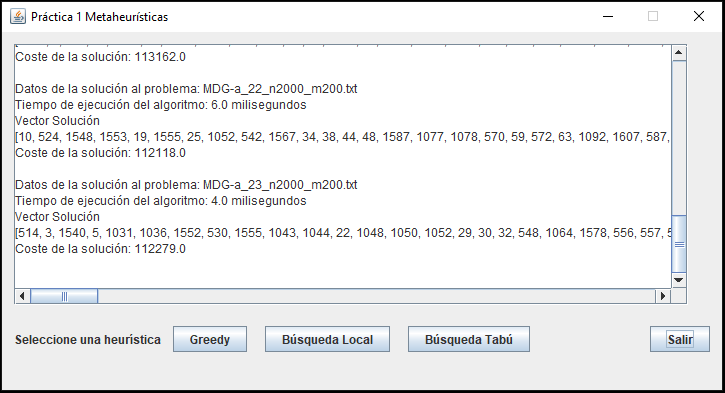
\includegraphics[scale=0.4]{img/GUI}
			\caption{GUI}
		
		\end{figure}
	
	\subsection{Parámetros de los algoritmos}
	
		\subsubsection{Greedy}
		
				\paragraph{}La heurística greedy toma como único parámetro la semilla, que se usa para generar el primer elemento de la solución, por tanto es una heurística muy cercana a un procedimiento determinista.
	
		\subsubsection{Búsqueda Local}
		
			\begin{itemize}
				
				\item Criterio de parada : Cuando no se encuentra mejora en las soluciones vecinas.
				
				\item Criterio de movimiento: Se realiza un movimiento a la primera solución vecina que nos mejore (first-improvement rule).
				
			\end{itemize}
				
	
		\subsubsection{Búsqueda Tabú}
		
			\begin{itemize}
				
				\item Iteraciones tabú: 50000.
				
				\item Memoria a corto plazo: La lista tabú tiene una tenencia de 5 elementos.
				
				\item Intentos tabú: 300, número máximo de iteraciones sin mejora antes de aplicar la oscilación estratégica.
				
				\item Memoria a largo plazo: La memoria a largo plazo se ha diseñado como un vector de enteros, la memoria no se reinicializa al realizar oscilaciones estratégicas.
				
				\item Probabilidad de reinicio: La probabilidad de reinicio a la hora de realizar la oscilación estratégica viene dada por la función :
				
				\[ \frac{nIteraciones}{maxIteraciones} \]
				
				Se aplicará pasadas 300 iteraciones sin mejora.
				
				\item Entorno de búsqueda: El numero de vecinos a evaluar en cada iteración se calcula como:
				
				\[ e^{\frac{limitIter - nIte}{ \frac{limitIter}{\log{\emph{m}}}}}\]
					
			\end{itemize}
	
	\subsubsection{Semillas}
	
	\paragraph{}Para la generación de números pseudoaleatorios se utiliza una semilla previamente definida en el archivo de configuración, en este caso es 77356084. Esta semilla se va rotando en las 5 iteraciones de cada archivo.
	
	
	\paragraph{} 77356084 $\rightarrow$ 73560847 $\rightarrow$ 35608477  ...
	
	
	\subsection{Análisis de los resultados}
	
		\subsubsection{Greedy}
		
				\paragraph{}La heurística greedy tiene un comportamiento aceptable para los conjuntos de datos escogidos, es capaz de ofrecer unos resultados cercanos a los óptimos globales mientras mantiene unos tiempos mínimos.
			
			\begin{figure}[H]
				
				\centering
				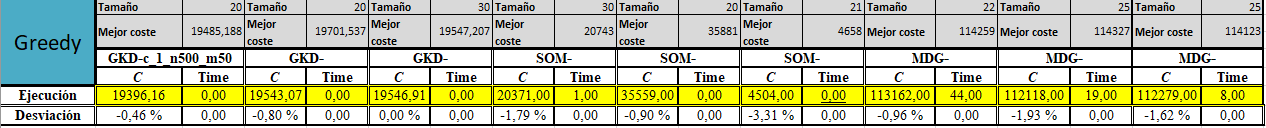
\includegraphics[scale=0.4]{img/greegyResult}
				\caption{Resultados obtenidos mediante Greedy}
				
			\end{figure}
		
			\begin{figure}[H]
				
				\centering
				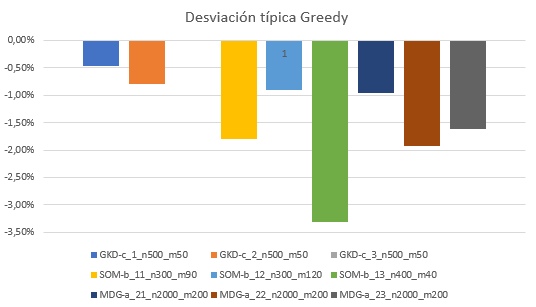
\includegraphics[scale=0.4]{img/DTGreedy}
				
			\end{figure}
		
			\begin{figure}[H]
				
				\centering
				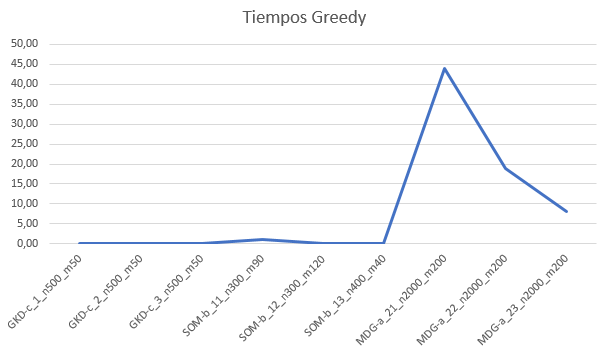
\includegraphics[scale=0.4]{img/TiemposGreedy}
				\caption{Tiempos expresados en milisegundos}
				
			\end{figure}
		
		\subsubsection{Búsqueda Local}
		
				\paragraph{}Como se puede observar en la tabla de resultados, la Búsqueda Local es muy robusta en los resultados, manteniendo unos tiempos comedidos. Esto puede deberse al hecho de que es un algoritmo muy simple, no obstante, esto lo puede llevar a caer en óptimos locales.
				
			 \paragraph{}La Búsqueda local es capaz de encontrar óptimos globales en algunos casos, a diferencia de Greedy, no obstante, los tiempos pueden llegar a ser 100 veces más lentos que los obtenidos en Greedy. Debido a la eliminación de la condición de parada basada en evaluaciones, las instancias pequeñas alcanzan el optimo local en torno a las 20000 evaluaciones, mientras que las instancias más grandes necesitan unas 300000.
				
			\begin{figure}[H]
				
				\centering
				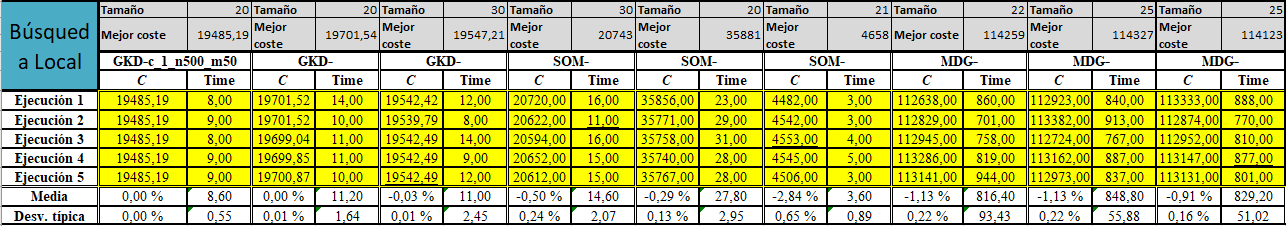
\includegraphics[scale=0.4]{img/blocalResult}
				\caption{Resultados obtenidos mediante Búsqueda Local}
				
			\end{figure}
		
		
			\begin{figure}[H]
				
				\centering
				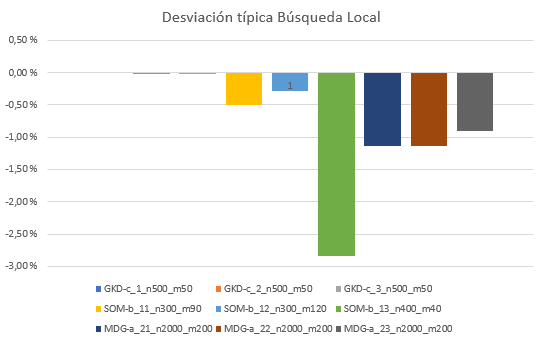
\includegraphics[scale=0.4]{img/DTBlocal}
				
			\end{figure}
		
			\begin{figure}[H]
				
				\centering
				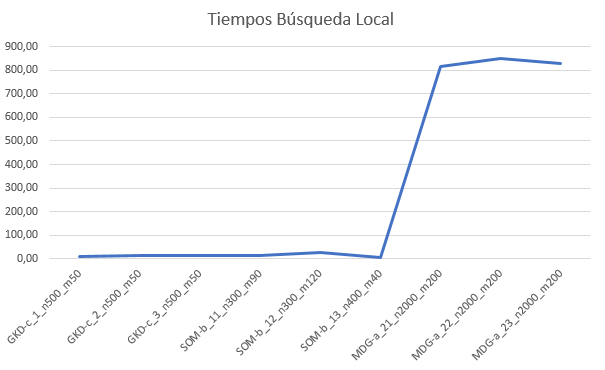
\includegraphics[scale=0.4]{img/TiemposBlocal}
				\caption{Tiempos expresados en milisegundos}
				
			\end{figure}
			
		\subsubsection{Búsqueda Tabú}
	
			\paragraph{}Para la Búsqueda Tabú se ha utilizado un sistema de memorias, aplicando una lista Tabú con tenencia de 5 iteraciones y una memoria de frecuencias basada en un vector de \emph{N} elementos, siendo \emph{N} el tamaño del problema. Realizando pruebas en base a aumentar la tenencia Tabú, hemos obtenido unos resultados en media similares, por tanto aumentar la tenencia Tabú no produce resultados significativos. Sin embargo, el aumento del número de iteraciones incrementa los resultados obtenidos, esto puede deberse al hecho de que el algoritmo dispone de más intentos de mejora desde soluciones creadas por la diversificación, permitiendo encontrar en algunos casos los óptimos globales.
			
			\paragraph{}Como se puede observar en los resultados, Búsqueda Tabú mejora en resultados a Búsqueda Local, esto es debido a que tiene capacidad de salir de óptimos locales, sin embargo, el aumento de tiempos es más que notable, obteniendo tiempos mayores para las instancias más pequeñas, que los obtenidos por Búsqueda Local en las instancias más grandes.
			
			\begin{figure}[H]
				
				\centering
				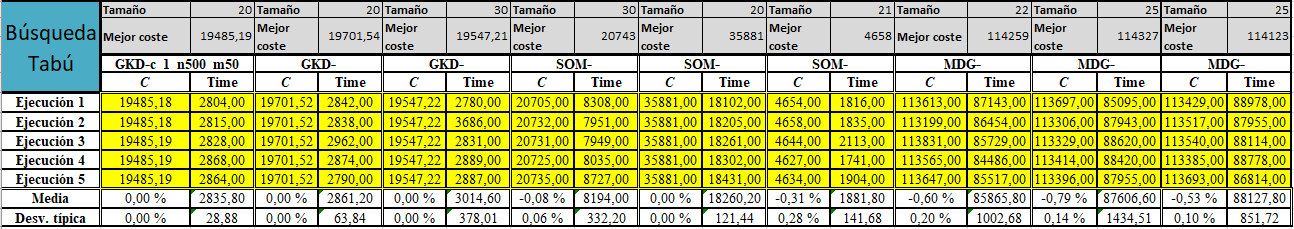
\includegraphics[scale=0.4]{img/btabuResult}
				\caption{Resultados obtenidos mediante Búsqueda Tabú}
				
			\end{figure}
		
			\begin{figure}[H]
				
				\centering
				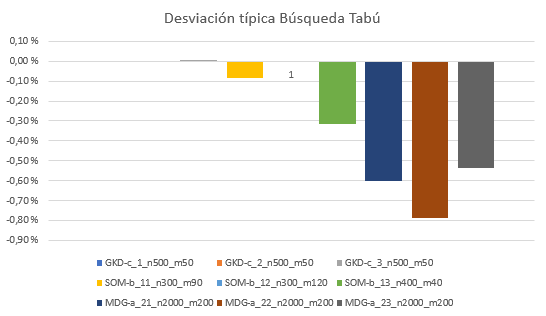
\includegraphics[scale=0.4]{img/DTBtabu}
				
			\end{figure}
		
			\begin{figure}[H]
				
				\centering
				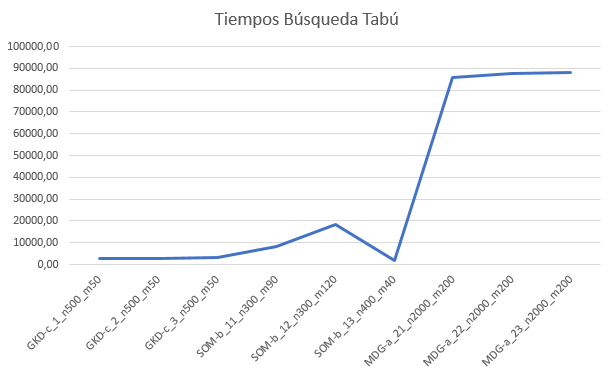
\includegraphics[scale=0.4]{img/TiemposBtabu}
				\caption{Tiempos expresados en milisegundos}
				
			\end{figure}
	
		\subsubsection{Comparativa entre algoritmos}
			
			
			\begin{figure}[H]
				
				\centering
				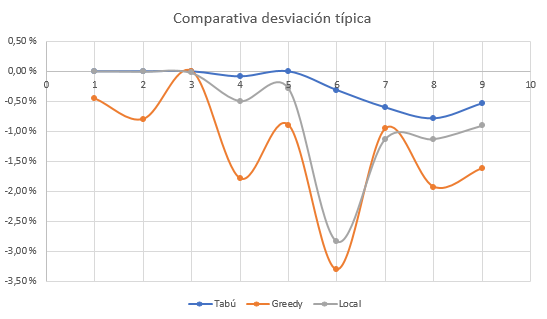
\includegraphics[scale=0.4]{img/DTGlobal}
				
			\end{figure}
			
			
			\begin{figure}[H]
				
				\centering
				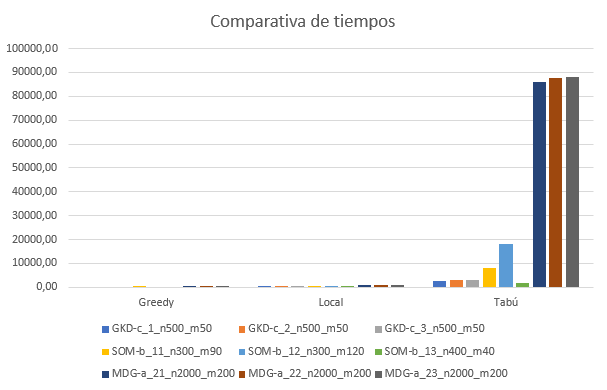
\includegraphics[scale=0.4]{img/TiemposGlobal}
				\caption{Tiempos expresados en milisegundos}
				
			\end{figure}
			


	\begin{thebibliography}{0}
		
		\bibitem{Glover2020} Fred Glover, Manuel Laguna, Rafael Martí. Principles of Tabu Search. https://www.uv.es/~rmarti/paper/docs/ts1.pdf
		
		\bibitem{UgrMe2020} https://sci2s.ugr.es/graduateCourses/Metaheuristicas
		
		\bibitem{UgrAl2020}https://sci2s.ugr.es/graduateCourses/Algoritmica
		
	\end{thebibliography}

\end{document}